\documentclass{article}

% Language setting
% Replace `english' with e.g. `spanish' to change the document language
\usepackage[english]{babel}

% Set page size and margins
% Replace `letterpaper' with`a4paper' for UK/EU standard size
\usepackage[letterpaper,top=2cm,bottom=2cm,left=3cm,right=3cm,marginparwidth=1.75cm]{geometry}

% Useful packages
\usepackage{amsmath}
\usepackage{graphicx}
\usepackage[colorlinks=true, allcolors=blue]{hyperref}
\usepackage{tikz}
\usetikzlibrary{arrows,matrix,positioning}

\title{PyLattice Notes}
\author{David Preti \\ \href{mailto:preti.david@gmail.com}{preti.david@gmail.com}}

\begin{document}
\maketitle


\section{Introduction}
This \texttt{python} package is intended for Lattice theories research. 

\section{Linear Algebra}
\subsection{Scalar}
\subsubsection*{\texttt{Real}}
\subsubsection*{\texttt{Complex}}

\subsection{Vectors}
\subsubsection*{\texttt{VectorReal}}
\subsubsection*{\texttt{VectorComplex}}

\subsection{Matrix}
\subsubsection*{\texttt{RealMatrix}}
\subsubsection*{\texttt{ComplexMatrix}}
\subsubsection*{\texttt{Identity}}

\subsection{Matrix Vector}
\subsubsection*{\texttt{VectorRealMatrix}}
\subsubsection*{\texttt{VectorComplexMatrix}}

\section{Lattice Objects}

\subsection{Lattice Scalar}
\subsubsection*{\texttt{LatticeReal}}
\subsubsection*{\texttt{LatticeComplex}}

\subsection{Lattice Matrix}
\subsubsection*{\texttt{LatticeRealMatrix}}
\subsubsection*{\texttt{LatticeComplexMatrix}}

\subsection{Lattice Vector}
\subsubsection*{\texttt{LatticeVectorReal}}
\subsubsection*{\texttt{LatticeVectorComplex}}

\subsection{Lattice Vector Matrix}
\subsubsection*{\texttt{LatticeVectorRealMatrix}}
\subsubsection*{\texttt{LatticeVectorComplexMatrix}}

\section{Parallelization}


\begin{figure}[t]
    \centering
        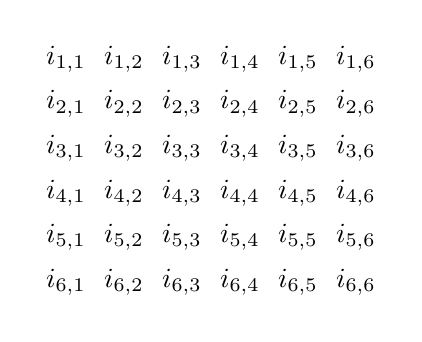
\begin{tikzpicture}
            \matrix [matrix of math nodes] (m)
                {
                    i_{1,1} & i_{1,2} & i_{1,3}  & i_{1,4} & i_{1,5} & i_{1,6} \\ 
                    i_{2,1} & i_{2,2} & i_{2,3} & i_{2,4} & i_{2,5} & i_{2,6} \\ 
                    i_{3,1} & i_{3,2} & i_{3,3} & i_{3,4} & i_{3,5} & i_{3,6} \\ 
                    i_{4,1} & i_{4,2} & i_{4,3} & i_{4,4} & i_{4,5} & i_{4,6} \\ 
                    i_{5,1} & i_{5,2} & i_{5,3} & i_{5,4} & i_{5,5} & i_{5,6} \\ 
                    i_{6,1} & i_{6,2} & i_{6,3} & i_{6,4} & i_{6,5} & i_{6,6} \\ 
                    };
        \end{tikzpicture}  
        \hspace{0cm}
        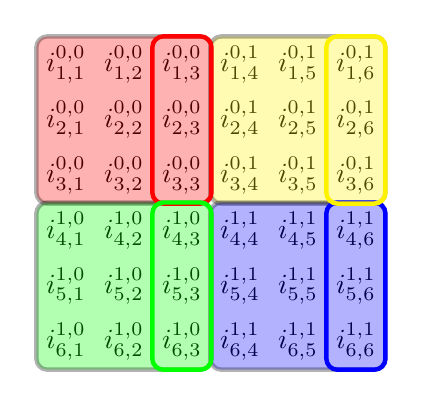
\begin{tikzpicture}
            \matrix [matrix of math nodes] (m)
            {
                i_{1,1}^{0,0} & i_{1,2}^{0,0} & i_{1,3}^{0,0} & i_{1,4}^{0,1} & i_{1,5}^{0,1} & i_{1,6}^{0,1} \\ 
                i_{2,1}^{0,0} & i_{2,2}^{0,0} & i_{2,3}^{0,0} & i_{2,4}^{0,1} & i_{2,5}^{0,1} & i_{2,6}^{0,1} \\ 
                i_{3,1}^{0,0} & i_{3,2}^{0,0} & i_{3,3}^{0,0} & i_{3,4}^{0,1} & i_{3,5}^{0,1} & i_{3,6}^{0,1} \\ 
                i_{4,1}^{1,0} & i_{4,2}^{1,0} & i_{4,3}^{1,0} & i_{4,4}^{1,1} & i_{4,5}^{1,1} & i_{4,6}^{1,1} \\ 
                i_{5,1}^{1,0} & i_{5,2}^{1,0} & i_{5,3}^{1,0} & i_{5,4}^{1,1} & i_{5,5}^{1,1} & i_{5,6}^{1,1} \\ 
                i_{6,1}^{1,0} & i_{6,2}^{1,0} & i_{6,3}^{1,0} & i_{6,4}^{1,1} & i_{6,5}^{1,1} & i_{6,6}^{1,1} \\ 
                };          
            \draw[rounded corners,ultra thick, draw=black, fill=red, opacity=0.3] (m-3-1.south west) rectangle (m-1-3.north east);
            \draw[rounded corners,ultra thick, draw=black, fill=green, opacity=0.3] (m-6-1.south west) rectangle (m-4-3.north east);
            \draw[rounded corners,ultra thick, draw=black, fill=yellow, opacity=0.3] (m-3-4.south west) rectangle (m-1-6.north east);
            \draw[rounded corners,ultra thick, draw=black, fill=blue, opacity=0.3] (m-6-4.south west) rectangle (m-4-6.north east);             
            \draw[rounded corners,ultra thick,draw=blue] (m-6-6.south west) rectangle (m-4-6.north east);
            \draw[rounded corners,ultra thick,draw=red] (m-3-3.south west) rectangle (m-1-3.north east);
            \draw[rounded corners,ultra thick,draw=yellow] (m-3-6.south west) rectangle (m-1-6.north east);
            \draw[rounded corners,ultra thick,draw=green] (m-6-3.south west) rectangle (m-4-3.north east);
        \end{tikzpicture}
        \hspace{0cm}
        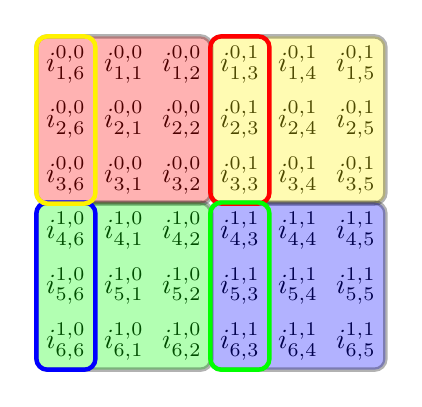
\begin{tikzpicture}
            \matrix [matrix of math nodes] (m)
            {
                i_{1,6}^{0,0} & i_{1,1}^{0,0} & i_{1,2}^{0,0} & i_{1,3}^{0,1} & i_{1,4}^{0,1} & i_{1,5}^{0,1} \\ 
                i_{2,6}^{0,0} & i_{2,1}^{0,0} & i_{2,2}^{0,0} & i_{2,3}^{0,1} & i_{2,4}^{0,1} & i_{2,5}^{0,1} \\ 
                i_{3,6}^{0,0} & i_{3,1}^{0,0} & i_{3,2}^{0,0} & i_{3,3}^{0,1} & i_{3,4}^{0,1} & i_{3,5}^{0,1} \\ 
                i_{4,6}^{1,0} & i_{4,1}^{1,0} & i_{4,2}^{1,0} & i_{4,3}^{1,1} & i_{4,4}^{1,1} & i_{4,5}^{1,1} \\ 
                i_{5,6}^{1,0} & i_{5,1}^{1,0} & i_{5,2}^{1,0} & i_{5,3}^{1,1} & i_{5,4}^{1,1} & i_{5,5}^{1,1} \\ 
                i_{6,6}^{1,0} & i_{6,1}^{1,0} & i_{6,2}^{1,0} & i_{6,3}^{1,1} & i_{6,4}^{1,1} & i_{6,5}^{1,1} \\ 
                };          
            \draw[rounded corners,ultra thick, draw=black, fill=red, opacity=0.3] (m-3-1.south west) rectangle (m-1-3.north east);
            \draw[rounded corners,ultra thick, draw=black, fill=green, opacity=0.3] (m-6-1.south west) rectangle (m-4-3.north east);
            \draw[rounded corners,ultra thick, draw=black, fill=yellow, opacity=0.3] (m-3-4.south west) rectangle (m-1-6.north east);
            \draw[rounded corners,ultra thick, draw=black, fill=blue, opacity=0.3] (m-6-4.south west) rectangle (m-4-6.north east);             
            \draw[rounded corners,ultra thick,draw=blue] (m-6-1.south west) rectangle (m-4-1.north east);
            \draw[rounded corners,ultra thick,draw=red] (m-3-4.south west) rectangle (m-1-4.north east);
            \draw[rounded corners,ultra thick,draw=yellow] (m-3-1.south west) rectangle (m-1-1.north east);
            \draw[rounded corners,ultra thick,draw=green] (m-6-4.south west) rectangle (m-4-4.north east);
        \end{tikzpicture}
        \label{fig:lattice-parallel1}
        \caption{Lattice partitioning for 4 processes. Halo boundaries are highlighted in the axis 1. }
\end{figure}

\begin{gather}
    idx(\mathbf{x},\mathsf{x}) %=\prod_d x_d+\alpha_d N_d + j \eta_d N_d
\end{gather}

\subsection{communication}
\subsection{I/O}

\texttt{LatticeBase}, \texttt{LatticeMPI}

\section{Example}
Ising Model

\end{document}